\section{پیش‌پردازش داده‌ها}
\label{sec:preprocessing}

مجموعه‌داده جمع‌آوری‌شده در شکل خام خود برای آموزش شبکه عصبی مناسب نیست. برای مثال، تعداد نقاط اندازه‌گیری‌شده در چرخه‌های مختلف یکسان نیست؛ درحالی‌که شبکه CNN به ورودی‌هایی با ابعاد مشخص و ثابت نیاز دارد.

\subsection{استخراج داده دشارژ و انتخاب ویژگی‌ها}

همان‌طور که پیش‌تر توضیح داده شد، به دلیل تفاوت در سیاست‌های شارژ، ابتدا اطلاعات مربوط به فرایند دشارژ باتری‌ها از مجموعه‌داده استخراج می‌شود. از میان پارامترهای ثبت‌شده، سه ویژگی اصلیِ ولتاژ، دما و ظرفیت دشارژ برای تشکیل ورودی شبکه عصبی انتخاب شده‌اند.

\subsection{یکسان‌سازی طول داده‌ها}

از آنجا که باتری‌های موجود در مجموعه‌داده با سیاست‌های شارژ متفاوتی آزمایش شده‌اند، برخی چرخه‌ها زودتر از چرخه‌های دیگر به پایان می‌رسند. بنابراین، زمان چرخه معیار مناسبی برای مقایسه ظرفیت دشارژ و دما در باتری‌های مختلف نیست. افزون بر این، زمان دشارژ به بار متصل و وضعیت سلامت باتری وابسته است. ازاین‌رو، به‌جای زمان، بازه ولتاژ به‌عنوان مرجع در نظر گرفته می‌شود. برای این منظور، بازه ولتاژ کاری (۳٫۶ تا ۲ ولت) به ۹۰۰ نقطه با فاصله‌های مساوی تقسیم می‌شود. مقدار هر ویژگی در هر نقطه ولتاژ، در صورت موجود بودن، مستقیماً از داده‌ها استخراج می‌شود؛ در غیر این صورت، مقدار آن با استفاده از درون‌یابی خطی به دست می‌آید. بدین ترتیب، برای هر چرخه از هر باتری، ۹۰۰ سطر حاوی اطلاعات ولتاژ، دما و ظرفیت دشارژ به دست می‌آید. نمونه‌ای از تغییرات دما و ظرفیت دشارژ بر حسب ولتاژ در شکل~\ref{fig:voltage} نمایش داده شده است. این نمودار نشان می‌دهد که ولتاژ می‌تواند به‌عنوان مرجع مشترکی برای استخراج مقادیر متناظر این ویژگی‌ها به کار رود.

\begin{figure}[!htbp]
\centering
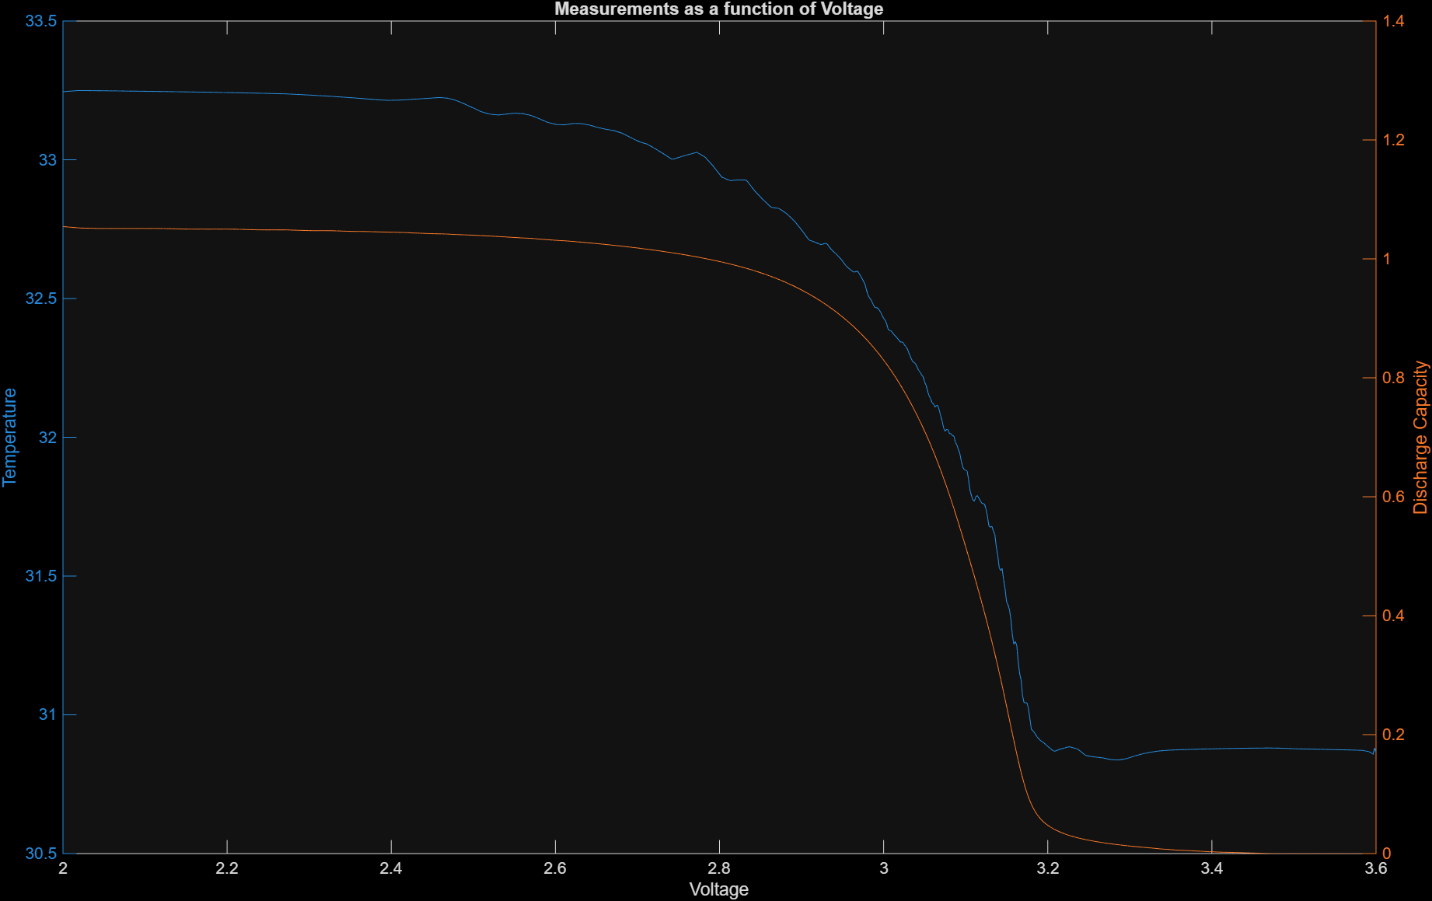
\includegraphics[width=0.9\textwidth]{img/voltage-ref.png}
\caption{تغییرات دما و ظرفیت دشارژ بر حسب ولتاژ در مرحله دشارژ یک چرخه؛ ولتاژ به‌عنوان مرجع مشترک برای استخراج مقادیر متناظر ویژگی‌ها در نظر گرفته شده است.}
\label{fig:voltage}
\end{figure}

\subsection{تبدیل به ماتریس سه‌کاناله}

در مرحله بعد، آرایه ۹۰۰ عضوی مربوط به هر یک از سه ویژگی به ماتریسی دوبعدی با ابعاد ۳۰ در ۳۰ تبدیل می‌شود؛در نتیجه، سه ماتریس دوبعدی با ابعاد یکسان به دست می‌آید. این ساختار مشابه یک تصویر رنگی با سه کانال اطلاعاتی است؛ با این تفاوت که هر کانال در اینجا یکی از ویژگی‌های ولتاژ، ظرفیت دشارژ یا دما را نمایش می‌دهد. تبدیل هر بردار ۹۰۰ عضوی به ماتریسی با ابعاد \(30\times30\)، این امکان را فراهم می‌کند که شبکه کانولوشنی الگوهای محلی میان عناصر مجاور ماتریس را استخراج کند. در واقع، فرض به‌کارگیری این ساختار آن است که الگوهای محلی حاصل از این بازآرایی می‌توانند برای پیش‌بینی عمر باتری مفید باشند.

\subsection{تعیین خروجی مورد انتظار شبکه}
\label{sec:target}

پس از آماده‌سازی داده‌های ورودی، لازم است خروجی مورد انتظار شبکه برای هر ورودی نیز تعیین شود؛ به بیان دیگر، باید مشخص شود شبکه برای هر ورودی چه مقداری را پیش‌بینی کند. هدف این پروژه، پیش‌بینی تعداد چرخه‌های باقی‌مانده عمر باتری بر اساس داده‌های یک چرخه است؛ بنابراین، خروجی مورد انتظار شبکه همان مقدار RUL خواهد بود. اگر باتری در مجموع $N$ چرخه تا رسیدن به پایان عمر خود داشته باشد، برای چرخه $i$ مقدار RUL مطابق رابطه~\eqref{eq:rul} محاسبه می‌شود:
\begin{equation}
\mathrm{RUL}_i = N - i + 1
\label{eq:rul}
\end{equation}

این مقدار مستقیماً به شبکه داده نمی‌شود. برای محدودکردن دامنه مقادیر خروجی، مقدار مورد انتظار با تقسیم بر عدد ثابت ۲۰۰۰ مقیاس‌بندی می‌شود. این عدد به‌عنوان ضریب مقیاس‌گذاری در پیاده‌سازی انتخاب شده و لزوماً نشان‌دهنده حداکثر طول عمر باتری در مجموعه‌داده نیست. رابطه~\eqref{eq:rulnorm} نحوه محاسبه مقدار نرمال‌شده RUL را نشان می‌دهد:
\begin{equation}
\widetilde{\mathrm{RUL}}_i = \frac{\mathrm{RUL}_i}{2000}
\label{eq:rulnorm}
\end{equation}

در نتیجه، برای هر چرخه دشارژ دو دسته اطلاعات در اختیار خواهد بود:
\begin{itemize}
\item ورودی: داده‌های ولتاژ، دما و ظرفیت دشارژ در قالب یک ماتریس $30 \times 30 \times 3$
\item خروجی: مقدار نرمال‌شده RUL
\end{itemize}

\subsection{تقسیم داده به آموزش، اعتبارسنجی و آزمون}
\label{sec:split}

در مرحله نهایی، داده‌های مربوط به ۴۰ باتری به سه مجموعه آموزش\LTRfootnote{Training}، اعتبارسنجی\LTRfootnote{Validation} و آزمون\LTRfootnote{Testing} تقسیم می‌شوند: مجموعه آموزش شامل ۳۰ باتری، مجموعه اعتبارسنجی شامل ۵ باتری و مجموعه آزمون نیز شامل ۵ باتری است. مجموعه آموزش برای یادگیری الگوهای موجود در داده‌ها، مجموعه اعتبارسنجی برای بررسی عملکرد مدل در طول فرایند آموزش و مجموعه آزمون برای ارزیابی نهایی مدل روی باتری‌هایی به کار می‌رود که در فرایند آموزش استفاده نشده‌اند. این تقسیم‌بندی به‌گونه‌ای انجام شده است که داده‌های مربوط به یک باتری به‌طور هم‌زمان در بیش از یک مجموعه قرار نگیرند.
